\documentclass[a4paper]{article}
\usepackage[estonian]{babel}
\usepackage[utf8]{inputenc}
\usepackage[T1]{fontenc}
\usepackage{mathtools}
\usepackage{amssymb,amsmath}
\usepackage{float}
\usepackage{siunitx}
\usepackage{graphicx}
\usepackage{pdfpages}
\usepackage{sidecap}
\graphicspath{ {./images/} }
\usepackage{geometry}
 \geometry{
 a4paper,
 total={170mm,257mm},
 left=20mm,
 top=20mm,
 }

\title{Valemid mahuti ruumala jaoks ja funktsioon MinuPytt}
\author{Siim Erik Pugal}
%\date{13. oktoober 2017. a}


\begin{document}
\maketitle

\section*{Sissejuhatus}
 Mahuti on jagatud kolmeks osaks, millest kaks on koonuse kujulised ja keskmine osa silndri kujuga. Valemid silindri ja koonuste jaoks on tuletatud kahes osas, et leida, mis on mahutis oleva vee ruumala.

\section*{Silindri ruumala}
 Idee mahuti keskmise osa ehk silindri ruumala leidmiseks on kogu silndri ruumalast lahutada tühja osa ruumala, mida vesi mahutis ei täida.

\subsection*{Täissilindri ruumala}

\begin{flushleft}
\textit{Rajad Descartes'i koordinaatsüsteemis:}
\begin{center}
$-R \leq x \leq R,$
\break
$-\sqrt{R^2-x^2} \leq y \leq \sqrt{R^2-x^2},$
\break
$ 0 \leq z \leq L.$
\end{center}
\end{flushleft}


\begin{equation}
\iiint_E dV\ = \int_{-R}^{R}\int_{-\sqrt{R^2-x^2}}^{\sqrt{R^2-x^2}}\int_{0}^{L} \,dx\,dy\,dz = 2 L \int_{-R}^{R} \sqrt{R^2-x^2} \,dx = \pi R^2 L
\end{equation}

\subsection*{Tühja osa ruumala}

\begin{flushleft}
\textit{Rajad Descartes'i koordinaatsüsteemis:} (vt. Joonis 1.)
\begin{center}
$0 \leq x \leq \sqrt{R^2 - [y+(H-R)]^2},$
\break
$ 0 \leq y \leq 2 R - H,$
\break
$ 0 \leq z \leq L.$
\end{center}
\end{flushleft}

\begin{equation} 
\begin{split}
\iiint_E dV\ & = 2 \int_{0}^{L}\int_{0}^{2R-H}\int_{0}^{\sqrt{R^2 - [y+(H-R)]^2}} \,dx\,dy\,dz = 2 \int_{0}^{L} \,dz \int_{0}^{2R-H} \,dy \int_{0}^{\sqrt{R^2 - [y+(H-R)]^2}} \,dx =\\ & =2 L \int_{0}^{2R-H} \sqrt{R^2 - [y+(H-R)]^2} \,dy = L\bigg[\frac{\pi R^2}{2} - R^2\arcsin\bigg(\frac{H-R}{R}\bigg)-(H-R)\sqrt{2 H R-H^2}\bigg]
\end{split}
\end{equation}

\begin{figure}[h]
\caption{Silindri ristlõige XY-tasandis: integreerimisrajad silindri tühja osa jaoks}
\centering
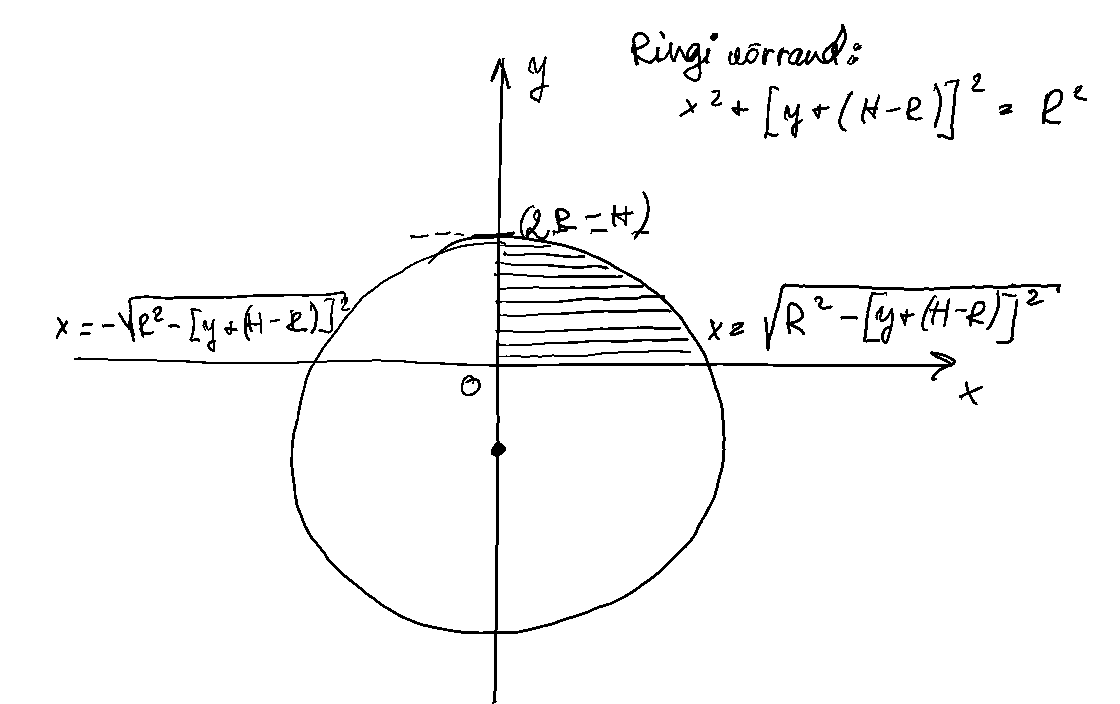
\includegraphics[width=0.5\textwidth]{silinder}
\label{fig:silinder}
\end{figure}

\subsection*{Silindrilise osa ruumala}
\begin{equation} 
\begin{split}
V & = \pi R^2 L - L\bigg[\frac{\pi R^2}{2} - R^2\arcsin\bigg(\frac{H-R}{R}\bigg)-(H-R)\sqrt{2 H R-H^2}\bigg]= \\ & = \frac{\pi R^2 L}{2} + L R^2\arcsin\bigg(\frac{H-R}{R}\bigg) + L (H-R)\sqrt{2 H R-H^2}
\end{split}
\end{equation}

 Antud kuju on valitud sellepärast, et funktsioonis $MinuPytt(R,L,l,H)$ saab väärtus $H$ olla vahemikus $0 \leq H \leq 2R$.

\vspace{7.5mm} %5mm vertical space

%\newpage

\section*{Koonuse ruumala}

\subsection*{Terve koonuse ruumala}

\begin{flushleft}
\textit{Descartes'i koordinaatides:} Rajad tulenevad lõputu koonuse valemist $R^2 z^2=l^2 x^2 + l^2 y^2$, mis avaneb z-telje positiivses suunas.
\begin{center}
$-R \leq x \leq R,$
\break
$-\sqrt{R^2-x^2} \leq y \leq \sqrt{R^2-x^2},$
\break
$ \frac{l}{R}\sqrt{x^2+y^2}\leq z \leq h.$
\end{center}
\end{flushleft}

% -\sqrt{R^2−x^2} \leq y \leq \sqrt{R^2−x^2}
% \frac{l}{R}\sqrt{x^2+y^2}\leq z \leq h
% -R \leq x \leq R}


\begin{equation} 
\begin{split}
V = \iiint_E dV\ & = \int_{-R}^{R}\int_{-\sqrt{R^2-x^2}}^{\sqrt{R^2-x^2}}\int_{\frac{l}{R}\sqrt{x^2+y^2}}^{h} \,dx\,dy\,dz = \\ &= \int_{-R}^{R} \,dx \int_{-\sqrt{R^2-x^2}}^{\sqrt{R^2-x^2}}\bigg(l - \frac{l}{R}\sqrt{x^2+y^2}\bigg) \,dy  = \\ & = \int_{-R}^{R} \,dx \int_{-\sqrt{R^2-x^2}}^{\sqrt{R^2-x^2}} h \,dy - \int_{-R}^{R} \,dx \int_{-\sqrt{R^2-x^2}}^{\sqrt{R^2-x^2}}\frac{l}{R}\sqrt{x^2+y^2} \,dy = \\ & = \pi R^2 l - \frac{2}{3} \pi R^2 l = \frac{1}{3} \pi R^2 l
\end{split}
\end{equation}

\subsection*{Osalise koonuse ruumala}

 Idee koonuse ruumala jaoks on kõigepealt tuletada valem, mis leiab ruumala poole koonuse ulatuses. Selle mõttekäik ja tuletus on sõnastatud järgnevalt:

\begin{center}
Koonuse kõrgus $= l$
\break
Koonuse põhja raadius $= R$
\break
Koonuse keskmise telje ja lõigitava pinna vaheline kaugus $= d, 0 \leq d \leq R$
\end{center}


\begin{flushleft}
Iga horisontaalne lõige on koonuses ringi kujuga. Need segmendid varieeruvad oma suuruse poolest, sest kui liikuda mööda koonust verikaalselt üles-alla, muutub ketta raadius. Oletame, et mingil kõrgusel $z$ on ringil raadius $r$, mis moodustab nurga $\theta$ ringi keskkohaga (vt. Joonis 2). Saame valemi
\end{flushleft}

\begin{figure}[H]
  \begin{minipage}{.35\textwidth}
\begin{equation}
\cos \bigg( \frac{\theta}{2} \bigg) = \frac{d}{r},
\end{equation}

 ehk

\begin{equation}
\theta = 2\arccos\bigg( \frac{d}{r} \bigg).
\end{equation}
  \end{minipage}%
  \begin{minipage}{.75\textwidth}
    \centering
    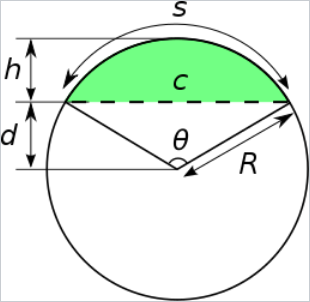
\includegraphics[width=0.4\textwidth]{koonus}
    \caption{Koonuse ristlõige XY-tasandis}
  \end{minipage}
\label{fig:koonus}
\end{figure}


%\begin{figure}[h]
%\caption{Koonuse ristlõige XY-tasandis.}
%\centering
%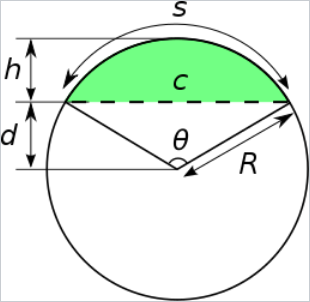
\includegraphics[width=0.75\textwidth]{koonus}
%\label{fig:koonus}
%\end{figure}

\begin{flushleft}
Olgu iga ketta paksus väljendatav seosega
\end{flushleft}

\begin{equation}
\,dz = \frac{l}{R} \,dr.
\end{equation}

\begin{flushleft}
Segmendi pindala:
\end{flushleft}

% Segmendi pindala
\begin{equation} 
\begin{split}
A & = \frac{r^2}{2} \big(\theta - \sin(\theta)\big)  = \frac{r^2}{2} \bigg[ 2\arccos\bigg( \frac{d}{r} \bigg) - \sin\bigg( 2\arccos\bigg( \frac{d}{r} \bigg) \bigg] \\ & =  r^2 \arccos\bigg( \frac{d}{r} \bigg) - d \sqrt{r^2 - d^2}.
\end{split}
\end{equation}

\begin{flushleft}
Seega on iga õhukese ketta ruumala väljendatav järgmise seosega:
\end{flushleft}

\begin{equation}
\,dV = A \,dz = A \frac{l}{R} \,dr = \frac{l}{R} \bigg( r^2 \arccos\bigg( \frac{d}{r} \bigg) - d \sqrt{r^2 - d^2} \bigg)\,dr .
\end{equation}

\begin{flushleft}
Ruumala avaldub seega järgmisel kujul:
\end{flushleft}

\begin{equation} \label{eq:9}
V = \int_{r=d}^{R} \frac{l}{R} \bigg( r^2 \arccos\bigg( \frac{d}{r} \bigg) - d \sqrt{r^2 - d^2} \bigg)\,dr
\end{equation}

\begin{flushleft}
Pärast seda kui Wolfram Mathematica minu arvutilt ligi 18 000 byte'i ära sõi, sai ta antud integraali vastuseks
\end{flushleft}

 
\begin{equation}
V = -\frac{d \cdot l}{2 R} \bigg[ \arccos\big(d^2 - R^2\big) + R\sqrt{R^2-d^2} + d^2 \log(d)-d^2\log\bigg(R + \sqrt{R^2 - d^2}\bigg) \bigg]
\end{equation}

\begin{flushleft}
See valem on peamiselt mõeldud kontrollimaks, kas meie rajad ja eeldused on korrektsed. Kui $d=0$, siis $V = \frac{1}{6}\pi R^2 l$ ning $d=R$ korral on $V=0$, seega on valem õigesti formuleeritud.
\vspace{2.5mm}

Kuna antud valem on pikk ja kohmakas ning $\log(d)$ võib väärtuse $d=0$ korral hakata koodis probleeme tekitama, jätan ma selle valemi Mathematica jaoks välja ning kasutan valemi ($\ref{eq:9}$) lahendamiseks Mathematicas funktsiooni $\texttt{NIntegrate[]}$.
\vspace{2.5mm}

Hetkel määrab vee taset koonuses muutuja $d$. Selleks, et see asendada muutujaga H on vaja tuua sisse kaks tingimust. Esiteks, kui veetase on koonuses vahemikus $0 \leq H \leq R$, siis omab muutuja $d$ kuju $d = R-H$. Teiseks: kui veetase on üle koonuse põhja raadiuse, siis on täiskoonuse ruumalast vaja maha lahutada tühja segmendi ruumala, mille korral hakkab kehtima tingimus $d = H-R$ ning koonuse ruumala hakatakse arvutama valemiga  
\end{flushleft}

\begin{equation}
\begin{aligned}
V = V_{Terve koonus} - V_{Poolkoonus} = 
\frac{\pi R^2 l}{6} -  \int_{d}^{R} \frac{l}{R} \bigg( r^2 \arccos\bigg( \frac{d}{r} \bigg) - d \sqrt{r^2 - d^2} \bigg)\,dr.
\end{aligned}
\end{equation}

\begin{flushleft}
Kuna koonused on mahuti mõlemas otsas kirjeldatavad samade parameetritega, siis on nad sümmeetrilised ning mahutuvuse poolest võrdväärsed. Seega on kogu mahuti ruumala kirjeldatav valemiga
\end{flushleft}

\begin{equation}
V_{Mahuti} = V_{Silinder} + 2 \cdot V_{Koonus} 
\end{equation}


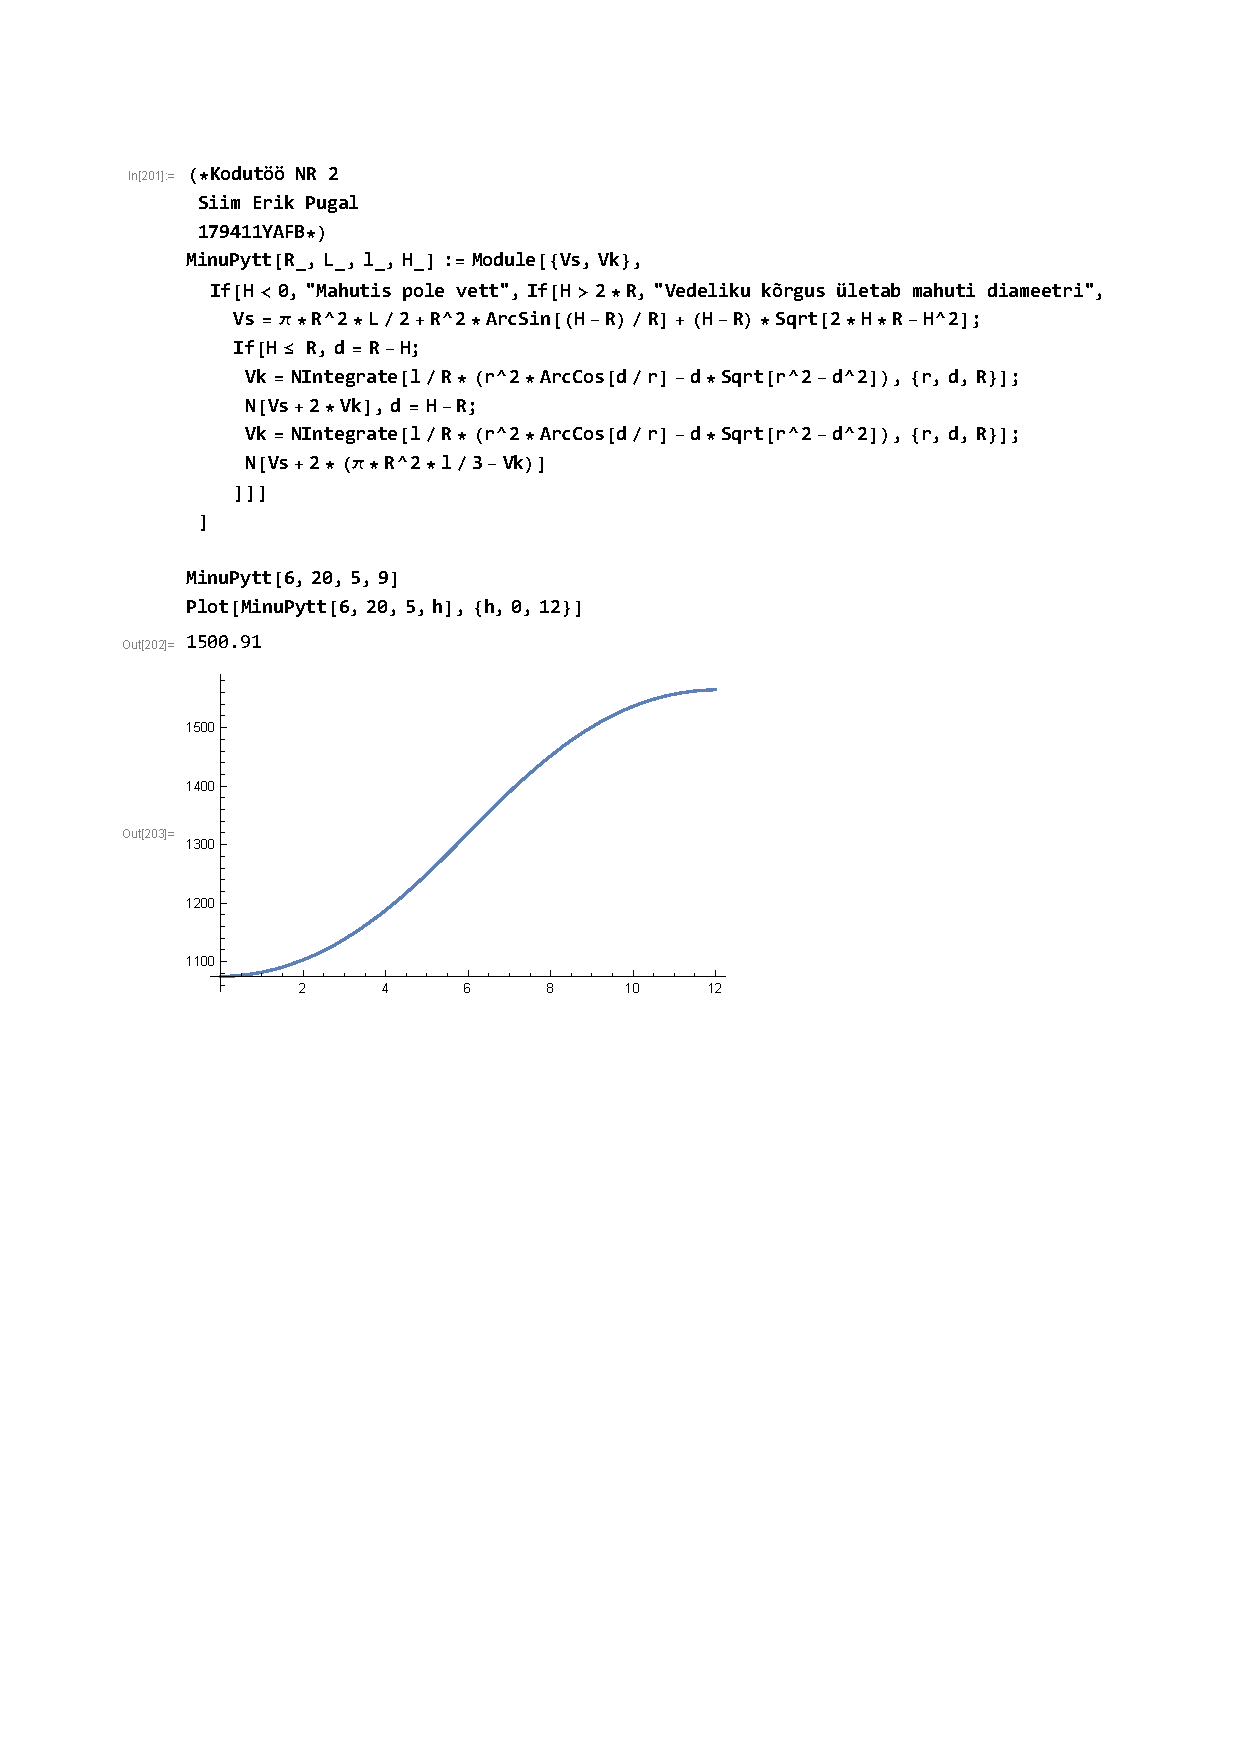
\includepdf{Kodutoo_nr2_Pugal}

\end{document}